\documentclass[11pt, a4paper, twoside]{ctexbook}
\usepackage{amsmath, amsthm, amssymb, bm, float,graphicx, geometry,hyperref, mathrsfs,amsopn}
\geometry{left = 2.54cm, right = 2.54cm, top = 3.18cm, bottom = 3.18cm}

\linespread{1.5}
\newtheorem{theorem}{定理}[section]
\newtheorem{definition}[theorem]{定义}
\newtheorem{lemma}[theorem]{引理}
\newtheorem{corollary}[theorem]{推论}
\newtheorem{example}[theorem]{例}
\newtheorem{proposition}[theorem]{命题}

\title{\textbf{数理方法复习}}
\author{Lvyangsen}
\date{\today}
\begin{document}
\maketitle

\setcounter{page}{0}
\newpage
\pagenumbering{Roman}
\setcounter{page}{1}
\tableofcontents
\newpage
\setcounter{page}{1}
\pagenumbering{arabic}

\newpage
\chapter{复变函数}
\section{基础}
\subsection{复数的几何表示、极坐标表示、指数表示}
模$\rho = \sqrt{x^2 +y^2}$, 辐角$\varphi = \arctan(\frac{y}{x})$
辐角主值$\mathrm{arg}z$, $\varphi = \mathrm{Arg} z = \mathrm{arg} z + 2k\pi(k = 0, \pm1,\pm 2, \cdots )$.
$$z = x + iy = \rho(\cos \varphi+ i\sin \varphi) = \rho e^{i\varphi}$$
\subsection{常见初等函数}
$$\begin{aligned}
    &e^z = e^x(\cos y + i \sin y) \qquad (\text{周期为}2\pi i)\\ 
    &\sin z = \frac{1}{2i}(e^{iz}-e^{-iz}) \qquad(\text{模可以大于1,周期为}2\pi)\\
    &\cos z = \frac{1}{2}(e^{iz}+e^{-iz})\\
    &\ln z = ln|z|+i\mathrm{Arg}z\qquad\text{(多值函数)}\\
    &z^s = e^{s\ln z}
\end{aligned}$$
\section{解析函数}
\begin{definition}[连续]
复变函数$f(z)$在点$z_0= x_0+ $i$y_0$连续的定义是:
$$
\begin{aligned}
    &\text{当 }z\to z_0\text{ 时,}f(z)\to f(z_0)\\
    &\text{即:}\forall\varepsilon>0,\quad \exists\delta(\varepsilon,z_0)>0\text{,使当 }|z-z_0|<\delta\text{ 时,恒有 }|f(z)-f(z_0)|<\varepsilon 
\end{aligned}
$$
\end{definition}
\begin{definition}[可导]
    单值函数$f(z)$在$z_0$点满足$\lim_{\Delta z\to0}\frac{f(z+\Delta z)-f(z)}{\Delta z}$存在,\\
    并且\underline{与$\Delta z \to 0$的方式无关},则称$f(z)$在$z_0$可导.
\end{definition}
\begin{definition}[解析]
    若 f(z) 在区域 G 内处处可导,则称 f(z) 是 G 内的解析函数。解析函数无穷阶可导
\end{definition}
\subsection{Cauchy-Riemann条件}

记$f( z) = f( x+ $i$y) = u( x, y) + $i$v( x, y)$
$$f(z)\text{在}z\text{点可导}\Rightarrow\frac{\partial u}{\partial x} = \frac{\partial v}{\partial y}, \quad \frac{\partial v}{\partial x} = -\frac{\partial u}{\partial y}$$

\textbf{极坐标形式:}$$\frac{\partial u}{\partial \rho}=\frac1\rho\frac{\partial v}{\partial\varphi},\qquad \frac1\rho\frac{\partial u}{\partial\varphi}=-\frac{\partial v}{\partial\rho}.$$

\textbf{充分必要条件:}
$$
f(z)\text{在}z\text{可导}\iff\begin{cases}\text{Cauchy-Riemann 条件}\\\frac{\partial u}{\partial x},\frac{\partial u}{\partial y},\frac{\partial v}{\partial x},\frac{\partial v}{\partial y}\text{存在且连续}\end{cases}
$$
\subsection{解析性质}
1. 若函数 $f( z) = u+ $i$v$ 在区域 $B$ 上解析,则
$$u(x,y)=C_1,v(x,y)=C_2$$
$(C_1,C_2$为常数)是$B$上的两组正交曲线族. 

2. 解析函数的实部和虚部都是调和函数,满足二维Laplace方程.
$$f(z)\text{解析}\implies\begin{cases}\nabla^2u=\frac{\partial^2u}{\partial x^2}+\frac{\partial^2 u}{\partial y^2}=0\\\nabla^2v=\frac{\partial^2 v}{\partial x^2}+\frac{\partial^2 v}{\partial y^2}=0\end{cases}$$
\begin{example}[由实部求虚部从而求出解析函数]
已知$u(x,y)$, $\Rightarrow \mathrm{d}v=-\frac{\partial u}{\partial y}\mathrm{d}x+\frac{\partial u}{\partial x}\mathrm{d}y.$ \\
\indent1. 可用曲线积分法(全微分的积分与路径无关)、不定积分法、凑微分法对$v = \int dv$进行求解。\\
2. 注意$f(z)$要最终表示为以$z$为自变量的形式,以及积分过程中不能忘记常数项$C$.\\
3. 可用极坐标系,注意使用极坐标系形式的柯西黎曼条件  \\
\end{example}
\section{多值函数}
详见吴崇试《数学物理方法》P22.
\begin{example}[根式函数]
    $$w = \sqrt{z-a}$$ 
    $$|w|=\sqrt{|z-a|},\quad\arg w=\frac{1}{2}\arg(z-a).$$
    $w$值的多值性来源于\underline{$z-a$辐角的多值性}.$w$值的多值性表现为辐角的多值性.我们称引起多值性的$z-a$为宗量.
    
    绕$a$点一周后,$\arg w$变化$\pi$,因此$w$变化$|w|e^{i\pi}$, $a$为分支点.
    \begin{figure}[htbp]
        \centering
        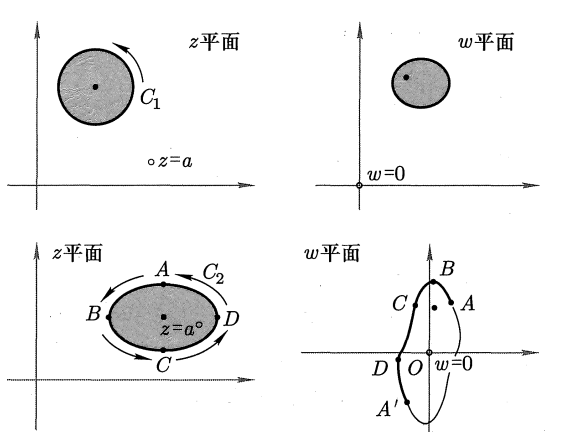
\includegraphics[width = 8cm]{多值函数.png}
        \caption{$z$沿闭合曲线一周回到原处时,$w= \sqrt{z-a}$值的不同变化}
    \end{figure}
    考察$z = \infty$是否为分支点, 设$z = \frac{1}{t}$, 考察$t = 0$是不是$f(t) = \sqrt{\frac{1-at}{t}}$的分支点.
    $t$绕着$\forall r < \frac{1}{|a|}$的圆$|t| = r$逆时针一周回到原处时,$\arg(1-at)$不变,但是$\arg t$增加$2\pi$,
    因此$\arg\sqrt{(1/t)- a}$减少$\pi$,因此$t = 0$为$f(\frac{1}{t})$的分支点,故而$z = \infty$为$f(z)$的分支点.
\end{example}
\begin{example}[对数函数]
    $$w = \ln z$$
    将$z = re^{i\theta}$,带入得$$w = \ln  r+ i(\theta + 2n\pi) + \ln|z| + i \mathrm{Arg}(z)$$
    对数函数$w$值的多值性来源于宗量$z$辐角的多值性,$w$值的多值性表现为$w$值虚部的多值性.
    对于每一个$z$值,有无穷多个$w$值,它们虚部相差$2\pi$的整数倍.
    $z = 0$与$z = \infty$为$w = \ln(z)$的分支点.
\end{example}
\renewcommand{\cleardoublepage}{}
\renewcommand{\clearpage}{}
\chapter{复变积分}
\section{复变积分}
\begin{definition}[复变积分]
  设$C$是$\mathbb{C}$内由A点到B点的曲线,函数$f(z)$在$C$上有定义,将$C$任意分割成$n$段,分点为$z_0(= A),z_1,z_2,\cdots,z_n(=B)$,$\zeta_k$是$z_{k-1} \to z_{k}$段上的任意一点,作和数,
若当$n\to\infty, \max|\Delta z_k|\to 0$时,此和数的极限存在,且极限值与$\zeta_k$的选取无关,则称此极限值为函数$f(z)$沿曲线的积分。
\end{definition}
$$\begin{aligned}\int_Cf(z)\mathrm{d}z=\int_C\left(u+\mathrm{i}v\right)\left(\mathrm{d}x+\mathrm{i}\mathrm{d}y\right)=\int_C\left(u\mathrm{d}x-v\mathrm{d}y\right)+\mathrm{i}\int_C\left(v\mathrm{d}x+u\mathrm{d}y\right).\end{aligned}$$
积分不等式:$$\left|\int_lf(z)\mathrm{d}z\right|\leqslant\int_l\left|f(z)\mid\mid\mathrm{d}z\right|$$.

\section{Cauchy 定理}
\subsection{单通连区域柯西定理}
如果函数$f(z)$在闭单连通区域$\overline{B}$上解析,则沿$\overline{B}$ 上任一分段光滑闭合曲线 $l( $也可以是$\overline B$ 的边界),有
$$
\oint_lf(z)\mathrm{~d}z=0.
$$
\subsection{复连通区域柯西定理}
如果$f(z)$是闭复连通区域上的单值解析函数,则
$$
\oint_lf(z)\mathrm{~d}z+\sum_{i\operatorname{=}1}^n\oint_{l_i}f(z\operatorname{)}\mathrm{~d}z=0\text{,}
$$
式中$l$为区域外边界线,诸$l_\mathrm{i}$为区域内边界线,积分均沿边界线的正方向进行,即沿$l$段为逆时针方向,而沿$l_1,l_2,\cdots,l_n$等段则为顺时
针方向.

\begin{theorem}
    (无论单连通还是多连通)如果函数$f(z)$在有界闭区域$\overline{G}$上解析,则沿$\overline{G}$的边界$C$,
    $$\boxed{\oint_C f(z) \mathrm{~d}z = 0}$$
\end{theorem}
\begin{example}
    计算积分$$I=\oint_{l}\left(z-\alpha\right)^{n}\mathrm{d}z\quad(n\text{ 为整数}).$$
    $$\begin{aligned}
    &\frac{1}{2\pi i }\oint_l \frac{\mathrm{d} z}{z - \alpha} = \begin{cases}&0, l\text{不包围}\alpha\\&1, l\text{包围}\alpha\end{cases}\\
    &\oint_l (z-\alpha)^n \mathrm{d}z = 0 \qquad(n \ne -1)
    \end{aligned} $$
\end{example}
\subsection{不定积分}
\begin{corollary}
    若 $f(z)$ 在有界单连通区域 $G$ 中解析,则复变积分 $\int _Gf( z) $d$z$ 与路径 $C$ 无关,其中$C\subset G$.
\end{corollary}
由此推论可以定义单值的不定积分.
\begin{theorem}[不定积分的解析性]
    若函数$f(z)$在有界单连通区域$G$内解析,则$f(z)$的不定积分
    $$F(z) = \int_{z_0}^zf(\zeta)\mathrm{d}\zeta, z\in G$$
    也在$G$内解析.
\end{theorem}
\section{小圆弧和大圆弧引理}
\begin{corollary}[小圆弧引理]
    如果函数 $f(z)$ 在 $z=a$ 点的空心邻域内连续,并且在 $\theta_1\leqslant$
    $\arg(z-a)\leqslant\theta_2$ 中,当$|z-a|\to0$ 时,$(z-a)f(z)$ 一致地趋近于 $k$,则
    $$\boxed{\lim_{\delta\to0}\int_{C_\delta}f(z)\mathrm{d}z=\mathrm{i}k(\theta_2-\theta_1)}$$
\end{corollary}
\begin{corollary}[大圆弧引理]
    设 $f(z)$ 在 $\infty$ 点的邻域内连续,在 $\theta_1\leqslant\arg z\leqslant\theta_2$ 中,当 $|z|\to\infty$ 时,$zf(z)$ 一致地趋近于$K$,则
    $$\lim_{R\to \infty} \int _{C_R} f(z)\mathrm{d}z = iK(\theta_2-\theta_1)$$
\end{corollary}
\section{Cauchy 积分公式}
\subsection{有界闭区域}
设 $f(z)$ 是\underline{有界闭区域 $\overline{G}$ 中的单值解析函数},
$\overline{G}$ 的边界 $C$ 是分段光滑曲线,$a$ 为$G$ 内一点,则
$$\boxed{f(a)=\frac{1}{2\pi\mathrm{i}}\oint_C\frac{f(z)}{z-a}\mathrm{d}z,\quad a\in G},$$
其中积分路径沿 $C$ 的正向.

根据$a$的任意性,设$f(z)$在有界闭区域$\overline{G}$单值解析,$$f(z) = \frac{1}{2\pi i} \frac{f(\zeta)}{\zeta - z} \mathrm{d}\zeta,z\in G$$
\subsection{无界区域}
如果 $f(z)$ 在简单闭合围道 $C$ 上及 $C$ 外解析,且当 $z\to\infty$ 时,$f(z)$ 趋于 K,则 Cauchy 积分公式
$$
f(a)=\frac{1}{2\pi\mathrm{i}}\oint_C\frac{f(z)}{z-a}\mathrm{d}z+K
$$
仍然成立,此处$a$为顺时针方向时所包含的区域内的一点,$K = \lim_{z\to \infty}f(z)$. 
\subsection{Cauchy 积分公式的高阶导数形式}
如果$f(z)$在有界闭区域$\overline{G}$中解析,则在$G$内$f(z)$的任何阶导数$f^{(n)}(z)$均存在,并且
$$f^{(n)}(z)=\frac{n!}{2\pi  i}\oint_C \frac{\zeta}{(\zeta-z)^{n+1}}\mathrm{d}\zeta, z\in G,$$
其中$C$是$\overline{G}$的正向边界.

\renewcommand{\cleardoublepage}{}
\renewcommand{\clearpage}{}
\chapter{级数展开}
\section{幂级数}

\textbf{柯西根值判别法:}
\begin{itemize}
    \item 若$\lim_{k \to \infty}\sqrt[k]{|a_k(z-z_0)^k|} < 1$,则绝对收敛,收敛半径$R = \frac{1}{\lim_{k \to \infty}\sqrt[k]{|a_k|}}$.
    \item 若$\lim_{k \to \infty}\sqrt[k]{|a_k(z-z_0)^k|} > 1$,则发散.
\end{itemize}
\textbf{达朗贝尔比值判别法:}
\begin{itemize}
    \item 若$\lim_{k \to \infty}\frac{|a_{k+1}(z-z_0)^{k+1}|}{|a_k(z-z_0)^k|} = \lim_{k \to \infty}|\frac{a_{k+1}}{a_k}||z-z_0| < 1$, 则绝对收敛,
    收敛半径$R = \lim_{k \to \infty}|\frac{a_k}{a_{k+1}}|$
    \item 若$\lim_{k \to \infty}\frac{|a_{k+1}(z-z_0)^{k+1}|}{|a_k(z-z_0)^k|} = \lim_{k \to \infty}|\frac{a_{k+1}}{a_k}||z-z_0| < 1$,则发散.
\end{itemize}

\section{解析函数的Tylor展开}
\begin{theorem}
    设$f(z)$在以$z_{0}$为圆心的圆$C_R$内解析,则对圆内的任意$z$点,$f(z)$
$$f(z)=\sum_{k=0}^\infty a_k\left(z-z_0\right)^k,(|z-z_0| < R)$$
其中
    $$a_k=\frac1{2\pi\mathrm{i}}\oint_{c_{R_1}}\frac{f(\zeta)}{\left(\zeta-z_0\right)^{k+1}}\mathrm{d}\zeta=\frac{f^{\left(k\right)}\left(z_0\right)}{k!},$$
    $C_{R_1}$为圆 $C_{R}$ 内包含 $z$ 且与 $C_{R}$ 同心的圆.
\end{theorem}
    证明要点:$$\frac{1}{\zeta-z}=\frac{1}{(\zeta-a)-(z-a)}=\frac{1}{\zeta-a}\sum_{n=0}^{\infty}\left(\frac{z-a}{\zeta-a}\right)^{n},\quad|z-a|<|\zeta-a|$$

\begin{enumerate}
    \item 收敛范围:设$b$为离$z_0$最近的奇点,则$f(z)$在圆$|z-z_0| < |b-z_0|$内处处解析,收敛半径$R = |b-z_0|$.
    \item Tylor展开具有唯一性.
    \item Tylor级数常见方法技巧:\begin{itemize}
    \item 对已知的函数展开线性组合变量代换,微商,积分
    \item 级数乘法
    \item 待定系数法
    \end{itemize}
\end{enumerate}

\textbf{在无穷远点的Taylor展开:}如果函数$f(z)$在$z = \infty$解析,则也可以在$z = \infty$展开成Tylor级数.

做变量替换$z = 1/t$,求$f(1/t)$在$t = 0$处的展开,收敛范围$|t| < r$,则$|z|>1/r$
\section{解析函数的Laurent展开}
\begin{theorem}
    设$f(z)$在环形区域$R_2<|z-z_0|<R_1$的内部单值解析,则对环域上任一点 $z,f(z)$ 可展为幂级数
$$f(z)=\sum_{k=-\infty}^\infty a_k\left(z-z_0\right)^k,R_2 < |z-z_0|<R_1$$
其中
$$
a_k=\frac1{2\pi\mathrm{i}}\oint_{c}\frac{f(\zeta)}{\left(\zeta-z_0\right)^{k+1}}\mathrm{d}\zeta\:,
$$
积分路径$C$ 为位于环域内按逆时针方向绕内圆一周的任一闭合曲线.
Laurent展开也具有唯一性.
\end{theorem}
\section{孤立奇点的分类}

\renewcommand{\cleardoublepage}{}
\renewcommand{\clearpage}{}
\chapter{留数定理}
\section{留数定理}
\begin{theorem}[留数定理]
  设有界区域 $G$ 的边界 $C$ 为分段光滑的简单闭合曲线. 若除有限个孤立奇点 $b_k,k=1,2,3,\cdots,n$ 外,函数 $f(z)$ 在 $G$ 内单值解析,在$\overline{G}$ 中连续,并且 $f(z)$ 在
边界 $C$ 上连续,则沿区域 $G$ 边界正向的积分
$$\boxed{\oint_C f(z)dz = 2\pi i \sum_{k = 1}^n \mathrm{res}f(b_k)}$$
  res $f(b_k)$ 称为 $f(z)$ 在 $b_k$ 处的留数,它等于 $f(z)$ 在孤立奇点 $b_k$ 的空心邻域内 Laurent 展开的系数$a_{-1}$
\end{theorem}
\begin{theorem}[无穷远点的留数]
    若$f(z)$在复平面上只有有限个奇点,除此之外全部解析,并且$\infty$为$f(z)$的孤立奇点,那么函数$f(z)$在所有点(包含无穷远点)留数为0.
    $$\sum_{i = 1}^k\mathrm{Res}f(b_k) + \mathrm{Res}f(\infty ) = 0$$
\end{theorem}
\subsubsection{留数的计算}
1. 若$z_0$是$f(z)$的$m$阶极点,则
$$\mathrm{Res}f(z_0) = a_{-1} = \frac{1}{(m-1)!}\lim_{z\to z_0}{\frac{d^{m-1}}{dz^{m-1}}[(z-z_0)^mf(z)]}$$
2. 特别地,当$m = 1$, $z=z_0$为一阶极点的情形时,$$\mathrm{Res} = a_{-1} = \lim_{z\to z_0}(z - z_0)f(z).$$
3. 当有理函数$f(z) =\frac{P(z)}{Q(z)}$且$P(z)$在$z_0$处解析,$z_0$为$Q(z)$一阶极点时,
$$\mathrm{Res}f(z_0) = \lim_{z\to z_0}(z-z_0)f(z)= \frac{P(z_0)}{Q'(z_0)}$$
\textbf{极点阶数:}
$z_0$为$f(z)$的$m$阶极点$\Longleftrightarrow$ 存在一个在在$z_0$处非零的解析函数$P(z)$,可以再在$z_0$的去心领域表示为$$f(z) = \frac{P(z)}{(z-z_0)^m}$$
\subsection{有理三角函数的积分}
$$I = \int_0^{2\pi} R(\cos\theta, \sin\theta)d\theta, \theta \in [0,2\pi],$$
其中,$R$为关于$\sin\theta,\cos\theta$的有理函数,在积分区间$[0,2\pi]$连续.
\subsection{无穷积分}
$$I = \int_{-\infty}^{\infty} f(x)dx$$
复变函数$f(z)$在实轴没有奇点,在上半平面除了有限个奇点外是解析的,当$z$在上半平面及实轴上时,$zf(z)\Rightarrow 0$.

\textbf{积分主值:}
$$v.p.\int_{-\infty}^{\infty} f(x)dx = \lim_{R\to +\infty}\int_{-R}^Rf(x)dx$$
\begin{figure}[htbp]
    \centering
    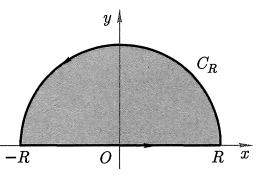
\includegraphics[width = 5cm]{无穷积分围道.png}
    \caption{无穷积分的典型围道}
\end{figure}
构造半圆围道$C$,半圆弧$C_R$,根据
$$\oint_{C}f(z)dz = \int_{C_R}f(z)dz + \int_{-R}^R f(x)dx = 2\pi i \sum_{C_R围道内}\mathrm{Res}{f(z)},$$
令$R\to \infty$,则$$\oint_{C}f(z)dz = 2\pi i \times \sum_{\text{上半平面}}\mathrm{Res}{f(z)}$$

$\lim_{R\to \infty}\int_{C_R}f(z)dz = 0$\textbf{的成立条件}
\begin{enumerate}
    \item 若$f(z) =\frac{P(z)}{Q(z)}$为有理函数,$\mathrm{deg}Q- \mathrm{deg}P \ge 2$
    \item  (大圆弧引理) 当$R\to \infty $时,$zf(z) \Rightarrow 0$(一致趋于0) 
\end{enumerate}
\subsection{含三角函数的无穷积分}
$\int_{0}^{\infty}F( x) \cos mx \mathrm{d}x, \int _0^\infty G( x) \sin mx\mathrm{d}x$. 积分区间是$[0,+\infty]$; 偶
函数$F(z)$和奇函数$G(z)$在实轴上没有奇点,在上半平面除有限个奇点外是解析的;当$z$在上半平面或实轴上$\to \infty$ 时,$F(z)$ 及 $G(z)$一致地$\Rightarrow 0$.

$$\int_0^{\infty}F(x)\cos mx dx = \frac{1}{2}\int_{-\infty}^{\infty} F(x)e^{imx}dx,F(x)\text{为偶函数} $$
$$\int_0^{\infty}G(x) \sin mx dx = \frac{1}{2 i}\int_{-\infty}^{\infty} G(x)e^{imx}dx,G(x)\text{为奇函数}$$

\begin{lemma}[Jordan引理]
    设在 0$\leqslant\arg z\leqslant\pi$ 范围内,当 $|z|\to\infty$ 时 $Q(z)$ 一致地趋于 0,则
    $$\lim_{R \to \infty}\int_{C_R} Q(z)e^{ipz}\mathrm{d}z = 0$$
其中 $p>0$, $C_R$ 是以原点为圆心,$R$ 为半径的上半圆弧.
\end{lemma}
\section{实轴上有单极点}
实轴上有有限个\underline{单极点}时,
$$\int_{-\infty}^\infty f(x)\operatorname{d}x=2\pi\mathrm{i}\sum_\text{上半平面}{ \operatorname { R e s }}f(z)+\pi\mathrm{i}\sum_\text{实轴上}{ \operatorname { R e s }} f(z).$$

\renewcommand{\cleardoublepage}{}
\renewcommand{\clearpage}{}
\chapter{傅里叶变换}
\section{傅里叶级数}
\subsection{正交函数系}
$$\begin{aligned}
    &\int_{-l}^l \cos\frac{k\pi x}{l} \sin\frac{n\pi x}{l} = 0\\
    &\int_{-l}^l \cos\frac{k\pi x}{l} \cos\frac{n\pi x}{l} = l\gamma \delta_{kn} = \begin{cases}&2l, k = n = 0\\&l,k = n \ne 0\\&0, k\ne n\end{cases}\\
    &\int_{-l}^l \sin\frac{k\pi x}{l} \sin\frac{n\pi x}{l} = l\delta_{kn}\begin{cases}&l,k = n\\&0,k \ne n\end{cases}
\end{aligned}$$
\subsection{周期函数的傅里叶级数}
$$\begin{aligned}
    &a_0 = \frac{1}{2l} \int_{-l}^l f(x)dx\\
    &a_n = \frac{1}{l}\int_{-l}^l f(x)\cos \frac{n\pi x}{l} dx, n \ne 0\\
    &b_n = \frac{1}{l}\int_{-l}^l f(x)\sin \frac{n\pi x}{l} dx\\
    &f(x) = a_0 + \sum_{n= 1}^{\infty}(a_n \cos\frac{n \pi x}{l} + b_n \sin \frac{n \pi x}{l})
\end{aligned}$$
\subsection{Dirichlet收敛定理}
\begin{theorem}
    若函数$f(x)$及其导数在一个积分周期内连续或者分段连续,只有有限个第一间断点(左右极限存在但不相等),则傅里叶级数在每一点都收敛,且
\begin{itemize}
    \item 若$x_0$为连续点,则傅里叶级数收敛到$f(x_0)$.
    \item 若$x_0$为间断点,则傅里叶级数收敛到$\frac{1}{2}(\lim_{x\to x_0^-}f(x) + \lim_{x\to x_0^+}f(x)).$
\end{itemize}
\end{theorem}
\subsection{复数形式的傅里叶级数}
$$\begin{aligned}
    &c_k = \frac{1}{2l}\int_{-l}^lf(\zeta)[e^{ik\omega\zeta}]^*\mathrm{d}\zeta\\
    &f(x) = \sum_{k = -\infty}^{\infty}c_ke^{ik\omega x}
\end{aligned}$$
\section{傅里叶积分变换}
\textbf{实数形式}
$$\begin{aligned}
    &A(\omega)= \frac{1}{\pi}\int_{-\infty}^{\infty}f(\varepsilon)\cos \omega \varepsilon \mathrm{d}\varepsilon\\
    &B(\omega)= \frac{1}{\pi}\int_{-\infty}^{\infty}f(\varepsilon)\sin \omega \varepsilon \mathrm{d}\varepsilon\\
    &f(x) = \int_0^{\infty}A(\omega)\cos \omega x \mathrm{d}\omega + \int_0^{\infty}B(\omega)\sin \omega x \mathrm{d}\omega
\end{aligned}$$
\textbf{复数形式}
$$\begin{aligned}
    &F(\omega) = \frac{1}{2\pi}\int_{-\infty}^{\infty}f(x)e^{-i\omega x}\mathrm{d}x\\
    &f(x) = \int_{-\infty}^{\infty}F(\omega)e^{i\omega x}\mathrm{d}\omega
\end{aligned}$$

\section{傅里叶复数变换的性质}
若$\mathscr{F}[f(t)] = F(\omega)$
\begin{enumerate}
    \item 线性 $$\begin{aligned}\mathscr{F}[\alpha f(t)+\beta g(t)]&=\alpha F(\omega)+\beta G(\omega)\\\mathscr{F}^{-1}[\alpha F(\omega)+\beta G(\omega)]&=\alpha f(t)+\beta g(t)\end{aligned}$$
    \item 延迟性 $$\mathscr{F}[f(t-t_0)]=e^{-i\omega t_0}F(\omega)$$
    \item 位移性 $$\mathscr{F}[e^{i\omega_0t}f(t)] = F(\omega-\omega_0)$$
    \item 相似性 $$\mathscr{F}[f(at)]=\frac1{|a|}F\left(\frac\omega a\right)$$
    \item 微分关系 $$\begin{gathered}\begin{aligned}\mathscr{F}\left[\frac{d^nf(t)}{dt^n}\right]=(i\omega)^nF(\omega)\end{aligned} \\\begin{aligned}\mathscr{F}^{-1}\left[\frac{d^nF(\omega)}{d\omega^n}\right]=(-it)^nf(t)\end{aligned} \end{gathered}$$
    \item 积分关系 $$\mathscr{F}[\int f(t)\mathrm{d}t]=\frac1{i\omega}F(\omega)$$
\end{enumerate}
\subsection{卷积}
\begin{definition}
    $$f_1(t)*f_2(t)=\int_{-\infty}^{+\infty}f_1(\tau)f_2(t-\tau)d\tau $$
\end{definition}
\begin{theorem}[时域卷积定理]
    $$\begin{aligned}\text{若 }\mathscr{F}[f(t)]=F(\omega),\quad\mathscr{F}[g(t)]&=G(\omega)\text{,则}\\\mathscr{F}[f(t)*g(t)]&=F(\omega)G(\omega)\end{aligned}$$ 
\end{theorem}
\begin{theorem}[频率卷积定理]
    $$\begin{aligned}\text{若 }\mathscr{F}[f(t)]=F(\omega),\quad\mathscr{F}[g(t)]&=G(\omega)\text{,则}\\\mathscr{F}[f(t)g(t)]&=\frac{1}{2\pi}F(\omega)*G(\omega)\end{aligned}$$  
\end{theorem}
\section{脉冲函数和阶跃函数}
\renewcommand{\cleardoublepage}{}
\renewcommand{\clearpage}{}
\chapter{Laplace变换}
\begin{definition}[Laplace积分变换]

    正变换:$$\overline{f}(p) = \int_0^{\infty}f(t)e^{-pt}\mathrm{d}t,$$
    其中$p = \sigma + i \omega $, $e^{-pt}$成为Laplace变换的核.

    逆变换:$$f(t) = \frac{1}{2\pi i}\int_{\sigma-\infty}^{\sigma + \infty}\overline{f}(p)e^{ip}\mathrm{d}p.$$
    $$\overline{f}(p) = \mathscr{L}[f(t)], \quad f(t) = \mathscr{L}^{-1}[\overline{f}(p)]$$
\end{definition}
\section{初等函数的Laplace变换}
\begin{enumerate}
    \item 常值函数 $$\mathscr{L}[1] = \frac{1}{p}, Re(p) > 0$$
    \item 线性函数 $$\mathscr{L}[t] = \frac{1}{p^2}, Re(p) > 0$$
    \item 幂函数 $$\mathscr{L}[t^n] = \frac{n!}{p^{n+1}}$$
    \item 指数函数 $$\mathscr{L}[e^{st}] = \frac{1}{p-s}, Re(p) > Re(s)$$
    \item 三角函数 $$\mathscr{L}[\cos \omega t] = \frac{p}{p^2 +\omega^2},\quad\mathscr{L}[\sin \omega t] = \frac{\omega}{p^2 +\omega^2} $$
    \item 求导运算的推论 $$\mathscr{L}[tf] = -\frac{\mathrm{d}}{\mathrm{d}p}\mathscr{e}[f] = -\frac{\mathrm{d}}{\mathrm{d}p} \overline{f}(p), \quad \mathscr{L}[t^nf] = -\frac{\mathrm{d}^n}{\mathrm{d}p^n}\mathscr{L}[f] = -\frac{\mathrm{d}^n}{\mathrm{d}p^n} \overline{f}(p)$$ 
\end{enumerate}
\begin{example}
    $$\mathscr{L}\left[t\mathrm{e}^{st}\right] = \frac{1}{(p-s)^2}, Re(p) > Re(s)$$
\end{example}
\section{Laplace变换的性质}

\begin{enumerate}
    \item 线性
    \item 导数性质 $$\begin{aligned}&\mathscr{L}[\mathrm{d}f/\mathrm{d}t] = p\mathscr{e}[f] - f(0)\\&\mathscr{e}[f^{(n)}] = p^n\mathscr{e}[f] - \sum_{i= 0}^{n-1}p^{n-1-i}f^(i)(0)\end{aligned}$$
    \item 积分性质 $$\mathscr{L}[\int_0^t f(\tau)\mathrm{d}\tau] = \frac{1}{p}\mathscr{e}[f(t)]$$
    \item 相似性 $$\mathscr{L}[f(at)] = \overline{f}(\frac{p}{a})$$
    \item 位移性 $$\mathscr{L}[e^{-\lambda}f(t)] = \overline{f}(p+\lambda)$$
    \item 延迟性 $$\mathscr{L}[f(t-t_0)H(t-t_0)] = e^{-pt_0}\overline{f}(p)$$
    \item 卷积 $$\mathscr{L}[f*g] = \mathscr{L}[f]\cdot\mathscr{L}[g]$$
    \item 初值定理 当$p\to \infty$时,$p\overline{f}(p)$极限存在,有$$f(0) = \lim_{p \to \infty}p \overline{f}(p)$$
    \item 终值定理  当$p\to 0$时,$p\overline{f}(p)$极限存在,有 $$f(0) = \lim_{p \to 0}p \overline{f}(p)$$
\end{enumerate}
Fourier变换和Laplace变换求解常微分方程和偏微分方程以及数理定界方程.

\chapter{定解方程的导出}
波动方程
两端固定:
$$u\mid_{x = 0} = 0, u\mid_{x = l} = 0$$
边界受力:
$$ES\frac{\partial u}{\partial n}=f(t)$$
自由即外力为0
$${\partial u}{\partial x}\mid_{x = 0} = 0$$
自由
绝热 $u_x = 0$
稳定恒定
自然边界条件

\chapter{数理定解方程求解方法}
\section{分离变量法}
\subsection{求解思路}
分离变量$\Rightarrow$求本征解$\Rightarrow$叠加$\Rightarrow$确定系数\\
(1) 对于泛定方程写出变量分离的形式解 $u(x,t)=X(x)T(t);$\\
(2) 代入泛定方程得到空间函数 $X(x)$ 和时间函数 $T(t)$ 的常微分方程;\\
(3) 求解 $X(x)$ 的常微分方程与相应的边界条件构成的本征值问题,得到本征值 $\lambda_n$ 和本征函数 $X_n(x);$\\
(4) 将 $\lambda_n$ 代入时间函数的方程解出 $T_n(t)$,与 $X_n(x)$ 相乘得到泛定方程的本征解 $u_n(x,t)=X_n(x)T_n(t);$\\
(5) 利用叠加原理得到一般解 $u(x,t)=\sum_{n=1}^{\infty}u_n(x,t)$, 并利用初始条件确定 $u_n(x,t)$ 中的系数。\\

\subsection{求解条件}
泛定方程必须\textbf{线性齐次},边界条件必须\textbf{齐次}.
\begin{example}[两端固定的弦自由振动]
    $$\left.\left\{\begin{array}{ll}\frac{\partial^2u}{\partial t^2}=a^2\frac{\partial^2u}{\partial x^2}&(0<x<L,t>0)\\\\u|_{t=0}=\phi(x),\quad\left.\frac{\partial u}{\partial t}\right|_{t=0}=\psi(x)&(0\leqslant x\leqslant L)\\\\u|_{x=0}=0,\quad u|_{x=L}=0&(t>0)\end{array}\right.\right.$$
\end{example}
\begin{example}[阻尼波动方程]
    $$\left.\left\{\begin{array}{ll}\frac{\partial^2u}{\partial t^2}-a^2\frac{\partial^2u}{\partial x^2}+2b\frac{\partial u}{\partial t}=0&(0<x<L,t>0)\\\u|_{t=0}=\phi(x),\quad\left.\frac{\partial u}{\partial t}\right|_{t=0}=\psi(x)&(0\leqslant x\leqslant L)\\\\u|_{x=0}=0,\quad u|_{x=L}=0&(t>0)\end{array}\right.\right.$$
\end{example}
\subsection{求解波动方程和输送方程的要点}
(1) 对于有界空间 ($0\leqslant x\leqslant L)$ 的波动方程与热传导方程的定解问题,其泛定方程具有变量分离的形式解 $u(x,t)=X(x)T(t)$,其中空间函数 $X(x)$ 所满足的方程在一般情况下具有确定的形式 $X^{\prime\prime}(x)+\lambda X(x)=0$,并与 $x=0$ 和 $x=L$ 两端的齐次边界条件结合,构成相关的本征值问题。本征值问题的解依赖于分离常数 $\lambda$ 的取值
 
$$\begin{aligned}
    &X(x)=A\cos kx+B\sin kx, \lambda > 0, k = \sqrt{\lambda}\\
    &X(x) = A + Bx, \lambda = 0\\
    &X(x) = A\cosh kx + B \sinh kx, \lambda < 0, k = \sqrt{-\lambda} 
\end{aligned}$$

(2)边界条件的组合
$$\overline{\begin{aligned}u_{x=0}&=0,\quad u_{x=L}=0:\lambda_n=\left(\frac{n\pi}L\right)^2,\quad Xn(x) = B_nsin(\frac{n\pi}{L}), \quad n = 1,\quad2,\quad3,\cdots\\\left.\frac{\partial u}{\partial x}\right|_{x=0}&=0,\left.\frac{\partial u}{\partial x}\right|_{x=L}=0:\lambda_n=\left(\frac{n\pi}L\right)^2,\quad X_n(x)=A_n\cos\frac{n\pi}Lx,\quad n=0,\quad1,\quad2,\cdots\\\left.u\right|_{x=0}&=0,\left.\frac{\partial u}{\partial x}\right|_{x=L}=0:\lambda_n=\left[\frac{(2n+1)\pi}{2L}\right]^2,\quad X_n(x)=B_n\sin\frac{(2n+1)\pi}{2L}x,\quad n=0,\quad1,\quad2,\cdots\\\left.\frac{\partial u}{\partial x}\right|_{x=0}&=0,\quad u|_{x=L}=0:\lambda_n=\left[\frac{(2n+1)\pi}{2L}\right]^2,\quad X_n(x)=A_n\cos\frac{(2n+1)\pi}{2L}x,\quad n=0,\quad1,\quad2,\cdots\\\hline\end{aligned}}$$
\section{本征函数法}
\subsection{适用对象}
边界条件齐次,与分离变量法同,但可求解非齐次线性泛定方程.
\subsection{求解思路}
对于非齐次方程,本征函数集的选择由相应得齐次方程和定解问题的边界条件确定.\\
(1)根据边界条件选择本征函数集,写出定解问题的级数形式解.\\
(2)将它代入泛定方程得到展开系数$T_N(t)$所满足得常微分方程.\\
(3)解出$T_n(t)$后,代入形式解并利用初始条件确定系数.
\subsection{泊松方程的定解问题}
\begin{example}[有源的稳态二维热传导]
   
\end{example}
对于非齐次的泊松方程,需要找出特解。
\newpage{}
\end{document}
